\documentclass[UTF8,a4paper,10pt]{ctexbook}

\usepackage[left=2.50cm, right=2.50cm, top=2.50cm, bottom=2.50cm]{geometry} %页边距
\CTEXsetup[format={\Large\bfseries}]{section} %设置章标题居左   
\usepackage{ctex}
\CTEXoptions[today=old]
\usepackage{cite}
\usepackage{textcomp}
\usepackage{listings}
\usepackage{xcolor}
\usepackage{varioref}
\usepackage{ctex}
\usepackage{multicol}
\usepackage{amssymb} 
\usepackage{setspace}
\usepackage{tikz} 
\usepackage{mdframed}
\usepackage{titletoc}
\usepackage{etoolbox}

\usepackage{helvet}
\usepackage{caption}
\usepackage{multicol} 
\usepackage{changepage}
\usepackage{graphics}
\usepackage{amsmath, amsfonts, amssymb}
\usepackage[english]{babel}
\usepackage{color}      
\usepackage{graphicx}   
\usepackage{url}        
\usepackage{bm}         
\usepackage{multirow}
\usepackage{booktabs}
\usepackage{epstopdf}
\usepackage{epsfig}
\usepackage{algorithm}
\usepackage{algorithmic}
\usepackage{listings}  % 代码框


\usepackage{listings}
\usepackage{color}

\definecolor{dkgreen}{rgb}{0,0.6,0}
\definecolor{gray}{rgb}{0.5,0.5,0.5}
\definecolor{mauve}{rgb}{0.58,0,0.82}

\lstset{ %
  language=C++,                % the language of the code
  basicstyle=\footnotesize,           % the size of the fonts that are used for the code
  numbers=left,                   % where to put the line-numbers
  numberstyle=\tiny\color{gray},  % the style that is used for the line-numbers
  stepnumber=1,                   % the step between two line-numbers. If it's 1, each line 
                                  % will be numbered
  numbersep=5pt,                  % how far the line-numbers are from the code
  backgroundcolor=\color{white},      % choose the background color. You must add \usepackage{color}
  showspaces=false,               % show spaces adding particular underscores
  showstringspaces=false,         % underline spaces within strings
  showtabs=false,                 % show tabs within strings adding particular underscores
  frame=single,                   % adds a frame around the code
  rulecolor=\color{black},        % if not set, the frame-color may be changed on line-breaks within not-black text (e.g. commens (green here))
  tabsize=2,                      % sets default tabsize to 2 spaces
  captionpos=b,                   % sets the caption-position to bottom
  breaklines=true,                % sets automatic line breaking
  breakatwhitespace=false,        % sets if automatic breaks should only happen at whitespace
  title=\lstname,                   % show the filename of files included with \lstinputlisting;
                                  % also try caption instead of title
  keywordstyle=\color{blue},          % keyword style
  commentstyle=\color{dkgreen},       % comment style
  stringstyle=\color{mauve},         % string literal style
  escapeinside={\%*}{*)},            % if you want to add LaTeX within your code
  morekeywords={*,...}               % if you want to add more keywords to the set
}


\usepackage[pagestyles]{titlesec}
\renewcommand{\algorithmicensure}{ \textbf{Input:}} 
\renewcommand{\figurename}{图}
\newcommand{\upcite}[1]{\textsuperscript{\textsuperscript{\cite{#1}}}}

\newpagestyle{teststyle}{
  \sethead{\emph{姓名:冯学伟}}{\emph{\sectiontitle}}{\emph{第\thepage页}}
  \renewcommand{\makeheadrule}{
    \makebox[0pt][l]{\rule[-.3\baselineskip]{\linewidth}{.5pt}}
    \rule[-.4\baselineskip]{\linewidth}{.5pt}
  }
}
\usepackage{color}
\usepackage{subfigure}
\usepackage{changepage}
\usepackage{fancyhdr}   %设置页眉、页脚
\pagestyle{fancy}       %%%单线页眉
\fancyhead{}
\fancyhead[LO]{px4 learning}
\fancyhead[RO]{fengxuewei}
\fancypagestyle{plain}{
  \pagestyle{fancy}
}
\usepackage[colorlinks,linkcolor=red]{hyperref}
\usepackage{shorttoc}
\usepackage{xcolor}
\usepackage{mdframed}
\usepackage{titletoc}

\DeclareRobustCommand{\chuhao}{\fontsize{42pt}{\baselineskip}\selectfont}  % 初号
\DeclareRobustCommand{\xiaochu}{\fontsize{36pt}{\baselineskip}\selectfont} % 小初
\DeclareRobustCommand{\yihao}{\fontsize{26pt}{\baselineskip}\selectfont}   % 一号
\DeclareRobustCommand{\xiaoyi}{\fontsize{24pt}{\baselineskip}\selectfont}  % 小一
\DeclareRobustCommand{\erhao}{\fontsize{22pt}{\baselineskip}\selectfont}   % 二号
\DeclareRobustCommand{\xiaoer}{\fontsize{18pt}{\baselineskip}\selectfont}  % 小二
\DeclareRobustCommand{\sanhao}{\fontsize{16pt}{\baselineskip}\selectfont}  % 三号 
\DeclareRobustCommand{\xiaosan}{\fontsize{15pt}{\baselineskip}\selectfont} % 小三
\DeclareRobustCommand{\sihao}{\fontsize{14pt}{\baselineskip}\selectfont}   % 四号
\DeclareRobustCommand{\xiaosi}{\fontsize{12pt}{\baselineskip}\selectfont}  % 小四
\DeclareRobustCommand{\wuhao}{\fontsize{10.5pt}{\baselineskip}\selectfont} % 五号
\DeclareRobustCommand{\xiaowu}{\fontsize{9pt}{\baselineskip}\selectfont}   % 小五
\DeclareRobustCommand{\liuhao}{\fontsize{7.5pt}{\baselineskip}\selectfont} % 六号
\DeclareRobustCommand{\xiaoliu}{\fontsize{6.5pt}{\baselineskip}\selectfont}% 小六
\DeclareRobustCommand{\qihao}{\fontsize{5.5pt}{\baselineskip}\selectfont}  % 七号

\lstset{numbers=left,numberstyle=\tiny,
breaklines=true,  %代码过长则换行
keywordstyle=\color{blue!70},commentstyle=\color{red!50!green!50!blue!50},frame=shadowbox, rulesepcolor=\color{gray!20!green!20!blue!20},escapeinside=``,xleftmargin=2em,xrightmargin=2em, aboveskip=1em}

\providecommand{\keywords}[1]{\textbf{\textit{keywords---}} #1}

% 设置章节格式
% 一级标题:黑体,三号,加粗;间距:段前 0.5 行,段后 1 行;
% \ctexset{chapter={
%     name = {第,章},
%     number = {\arabic{chapter}},
%     format = {\heiti \bfseries \centering \zihao{3}},
%     aftername = \hspace{9bp},
%     pagestyle = BIThesis,
%     beforeskip = 8bp,
%     afterskip = 32bp,
%     fixskip = true,
%   }
% }

% % 二级标题:黑体,四号,加粗;间距:段前 0.5 行,段后 0 行;
\ctexset{section={
    number = {\thechapter.\hspace{4bp}\arabic{section}},
    format = {\heiti \raggedright \bfseries \zihao{4}},
    aftername = \hspace{8bp},
    beforeskip = 20bp plus 1ex minus .2ex,
    afterskip = 18bp plus .2ex,
    fixskip = true,
  }
}

% % 三级标题:黑体、小四、加粗;间距:段前 0.5 行,段后 0 行;
\ctexset{subsection={
    number = {\thechapter.\hspace{3bp}\arabic{section}.\hspace{3bp}\arabic{subsection}},
    format = {\heiti \bfseries \raggedright \zihao{-4}},
    aftername = \hspace{7bp},
    beforeskip = 17bp plus 1ex minus .2ex,
    afterskip = 14bp plus .2ex,
    fixskip = true,
  }
}

% 设置目录样式
% 添加 PDF 链接
\addtocontents{toc}{\protect\hypersetup{hidelinks}}

% 解决「目录」二字的格式问题
\renewcommand{\contentsname}{
  \fontsize{16pt}{\baselineskip}
  \normalfont\heiti{目~~~~录}
  \vspace{-8pt}
}
% 定义目录样式
\titlecontents{chapter}[0pt]{\songti \zihao{-4}}
{\thecontentslabel\hspace{\ccwd}}{}
{\hspace{.5em}\titlerule*{.}\contentspage}
\titlecontents{section}[2\ccwd]{\songti \zihao{-4}}
{\thecontentslabel\hspace{\ccwd}}{}
{\hspace{.5em}\titlerule*{.}\contentspage}
\titlecontents{subsection}[4\ccwd]{\songti \zihao{-4}}
{\thecontentslabel\hspace{\ccwd}}{}
{\hspace{.5em}\titlerule*{.}\contentspage}

\usepackage{hyperref} %bookmarks
% \usepackage[colorlinks,linkcolor=red,anchorcolor=blue,citecolor=green,CJKbookmarks=True]{hyperref}
\hypersetup{colorlinks, bookmarks, unicode} % unicode
 
\captionsetup[figure]{labelfont={bf},labelformat={default},labelsep=period,name={图}}
\newenvironment{figurehere}
{\def\@captype{figure}}
{}

\title{
    \huge{\textbf{px4 learning}}
}

\author{fengxuewei}
\date{\today}

\begin{document}
    % \maketitle
    \tableofcontents
    \clearpage
    \pagestyle{teststyle}  
    px4: 代码结构清晰, 比较适合开发
    APM: 结构比较乱, 功能比较丰富, 稳定性好
    启动的时候需要sd卡里的一段引导程序,
    你要是把sd卡拔下来了飞控就启动不了了!还有就是是记录飞行日志和地形跟随的一些数据\par
    \chapter{flyMode}
\section{fly modes}
\begin{table}[h]
    \centering
    \caption{fly modes}\label{tab:tab2}
    \begin{tabular}{|c|c|}
    \hline
        MANUAL & \\\hline
        ACRO & \\\hline
        ALTCTL & \\\hline
        POSCTL & \\\hline
        OFFBOARD & \\\hline
        STABILIZED & \\\hline
        RATTITUDE  & \\\hline
        AUTO.MISSION & \\\hline
        AUTO.LOITER  & \\\hline
        AUTO.RTL  & \\\hline
        AUTO.LAND  & \\\hline
        AUTO.RTGS  & \\\hline
        AUTO.READY & \\\hline
        AUTO.TAKEOFF & \\\hline
    \end{tabular}
\end{table}
\clearpage
\section{takeOff}
\clearpage
\section{mission}
\clearpage
\section{landing}
\clearpage
\section{offboard}
\clearpage
\section{ALTCTL}
参数 \textcolor{red}{$NAV\_RCL\_ACT$}, 影响着最后的 Failsafe enabled: no RC 的错误警报. 
\begin{itemize}
    \item $NAV\_RCL\_ACT=0$: stop the fail safe behavior due to having no RC
\end{itemize}
\clearpage
    \clearpage
    \chapter{uorb}

\section{Single uorb}

    \subsection{advertise}
    \clearpage

    \subsection{publisher}
    \clearpage

    \subsection{subscriber}
    \clearpage

\section{Multiple uorb}

    \subsection{advertise}
    \clearpage

    \subsection{publisher}
    \clearpage

    \subsection{subscriber}
    \clearpage



    \clearpage
        导航就字面上说,就是引导航行的意思,而其确切的定义可表述为:导航是有目的地、
    安全有效地引导运动体(船只、潜艇、地面车辆以及飞机、宇宙飞船等). 也就是在当前位置已知的前提下,
    计算如何才能到达目的地,也即路径规划。本系统设计的导航子系统(navigator)执行流程如图\ref{fig:navigator}所示.
    \begin{figure}[htbp]
        \centering
        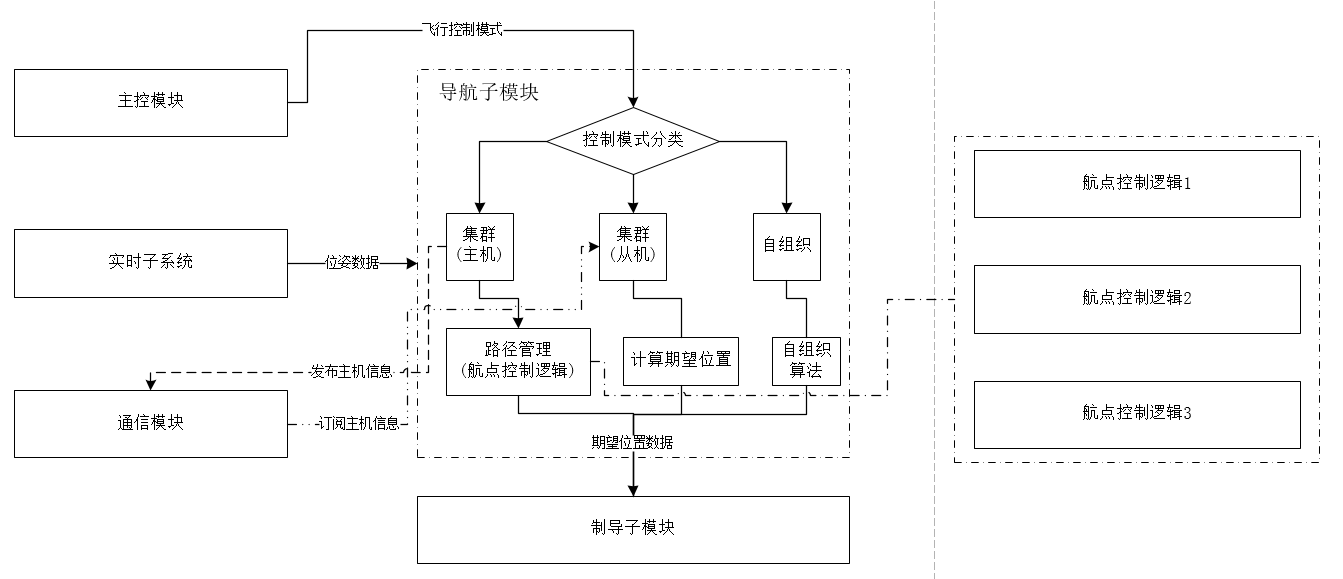
\includegraphics[width=\textwidth]{pictures/navigator.png}
        \caption{navigator}
        \label{fig:navigator}
    \end{figure}
    路径管理内部有三处控制逻辑, 分别对应着直线切换, 转弯圆角, 以及dubins曲线三种控制算法. 会在后面"算法"一节中进行介绍. 


    \clearpage
    \chapter{position controller}

\section{Single vehicle}
    \subsection{offboard control logic}

    \clearpage
    \subsection{vf control logic}
    
    \clearpage

\section{Multiple vehicles}
    \subsection{fomation control logic}

    \clearpage

\section{Publishing date to attitude controller}
    \clearpage
    \chapter{attitude controller}

\section{offboard}


\subsection{mavros发送offboard数据流}
\begin{lstlisting}[title=publish messgae, frame=shadowbox]
    // 1. offboard publish (mavros topic)
    fixed_wing_local_att_sp_pub = nh.advertise<mavros_msgs::AttitudeTarget>("mavros/setpoint_raw/attitude", 10);
    
    #define MAVLINK_MSG_ID_SET_ATTITUDE_TARGET 82
      typedef struct __mavlink_set_attitude_target_t {
          uint32_t time_boot_ms; /*< [ms] Timestamp (time since system boot).*/
          float q[4]; /*<  Attitude quaternion (w, x, y, z order, zero-rotation is 1, 0, 0, 0)*/
          float body_roll_rate; /*< [rad/s] Body roll rate*/
          float body_pitch_rate; /*< [rad/s] Body pitch rate*/
          float body_yaw_rate; /*< [rad/s] Body yaw rate*/
          float thrust; /*<  Collective thrust, normalized to 0 .. 1 (-1 .. 1 for vehicles capable of reverse trust)*/
          uint8_t target_system; /*<  System ID*/
          uint8_t target_component; /*<  Component ID*/
          uint8_t type_mask; /*<  Mappings: If any of these bits are set, the corresponding input should be ignored: bit 1: body roll rate, bit 2: body pitch rate, bit 3: body yaw rate. bit 4-bit 6: reserved, bit 7: throttle, bit 8: attitude*/
     }) mavlink_set_attitude_target_t;
\end{lstlisting}
\section{Coordinated Turn 协调转弯}
\subsection{not being wind}
方向角的变化率是和机体的roll以及倾斜角(bank angle)有关系, 我们需要寻找一个简单的关系来帮助我们研究这种线性传递函数的关系 -- 协调转弯. \par
在协调转弯期间, 飞机在体坐标系下没有横向加速度. 从分析的角度来看, 协调转弯的一个假设运行我们得到一个简单的表达式将 heading rate 和 bank angle 联系起来. \par
协调转弯时, 为了无人机没有侧向力, bank angle $\phi$ 被设置.
在图\ref{fig:1}中, 作用在微型飞行器上的离心力与作用在水平方向上的升力的水平分量相等并相反。
\begin{figure}[htpb]
    \centering
    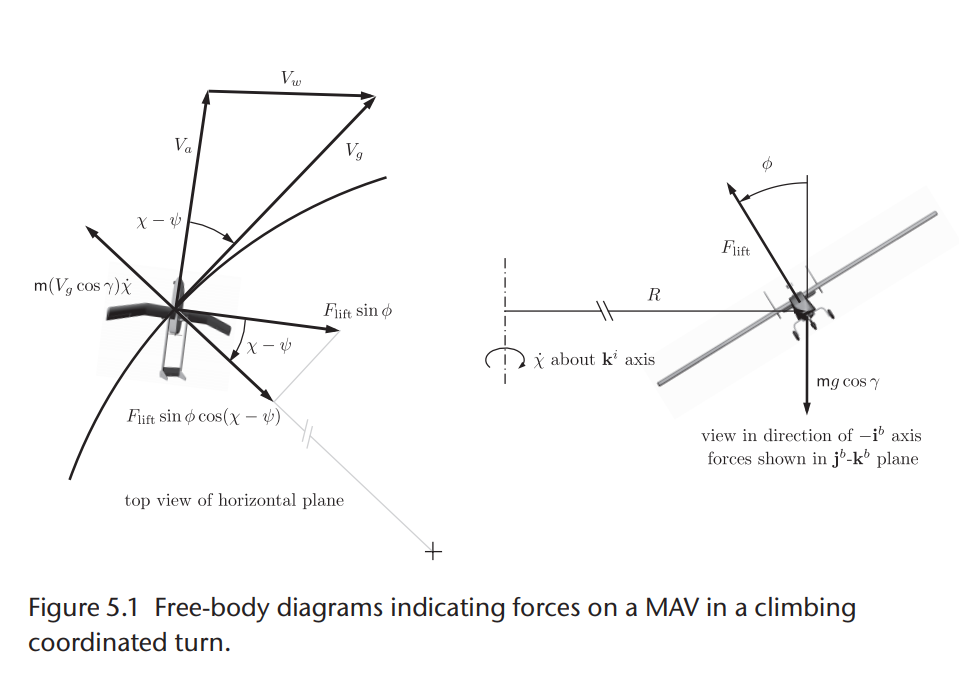
\includegraphics[width=0.8\textwidth]{pictures/5_1.png}
    \caption{爬升协调转弯MAV上的力}
    \label{fig:1}
\end{figure}
\par 作用在水平方向力的关系表示如下: 
\begin{align}
    F_{lift} sin \phi cos (\chi - \psi) &= m \frac{v^{2}}{R} \nonumber \\
    &= m v \omega \nonumber \\
    &= m (V_{g} cos \gamma) \dot{\chi} 
    \label{equ:1}
\end{align}
其中, $F_{lift}$代表的是升力, $\gamma$ 代表的是飞行轨迹的角度, $V_{g}, \chi$ 分别表示的是地速度以及方向角. \textcolor{red}{向心加速度的表达式: $a_{n} = \frac{v^{2}}{R} = v \omega$}
\par 离心力(The centrifugal force)(\textcolor{red}{$m (V_{g} cos \gamma) \dot{\chi} $})计算的时候, 用到了在惯性坐标系$k^{i}$上的方向角变化率$\dot{\chi}$ 和 速度的水平分量 $V_{a}cos \gamma$
\par 同样, 升力的垂直分量与重力在 $j^{b} - k^{b}$平面上的投影是等大反向的. 
垂直方向上的合力为:
\begin{equation}
    F_{lift} cos \phi = mg cos\gamma
    \label{equ:2}
\end{equation}
将等式\ref{equ:1}除以\ref{equ:2}得的 $\dot{\chi}$
\begin{equation}
    \dot{\chi} = \frac{g}{V_{g}} tan \phi cos(\chi - \psi)
    \label{equ:3}
\end{equation}
等式\ref{equ:3}就是协调转弯的表达式. 
\par 考虑到转弯半径等于 \textcolor{blue}{ $R = V_{g} \frac{cos \gamma}{\dot{\chi}}$}, 将上式代入半径中, 得到式子\ref{equ:4}. 在没有风或侧滑的情况下, 有\textcolor{red}{$V_{a} = V_{g}$和$\psi = \chi$}, 从而得到了式子\ref{equ:5}. 
\begin{equation}
    R = \frac{V_{g}^{2} cos \gamma}{g tan \phi cos(\chi - \psi)} 
    \label{equ:4}
\end{equation}
\begin{equation}
    \dot{\chi} = \frac{g}{V_{g}} tan \phi = \dot{\psi} = \frac{g}{V_{a}} tan \phi
    \label{equ:5}
\end{equation}
\par 在 9.2 节中, 我们将要介绍 在有风的情况下 \textcolor{blue}{$ \dot{\psi} = \frac{g}{V_{a}} tan \phi$} 该式子也成立
\clearpage
\subsection{being wind-Kinematic Model of Controlled Flight}
% 控制飞行动力学模型\par
在推导降阶表达式中, 简化的目的是估计运动中力平衡以及动量平衡的关系式(这些包含了 $\dot{u}, \dot{v}, \dot{\omega}, \dot{p}, , \dot{q}, \dot{r}$), 预估这些变量需要计算复杂的空气动力. 这些变量表达式可以被更简单的动力学表达式替代. 
这个更简单的动力学表达式是\textcolor{blue}{针对协调转弯和加速爬升的特定飞行条件而导出}.
\begin{figure}[htpb]
    \centering
    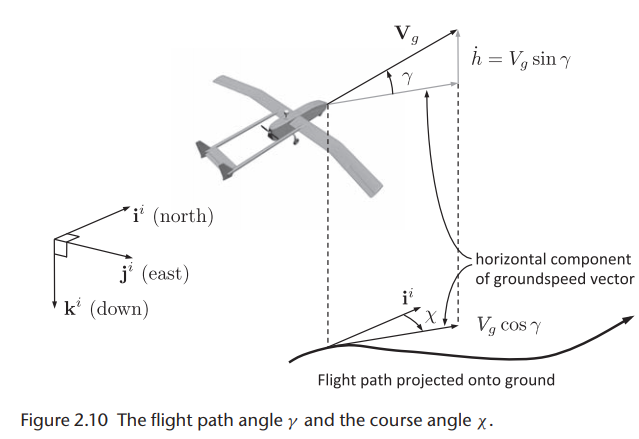
\includegraphics[width=0.8\textwidth]{pictures/2_10.png}
    \caption{航线轨迹角度$\gamma$和航向角$\chi$}
    \label{fig:2_10}
\end{figure}
针对图\ref{fig:2_10}, 飞机相对于惯性系的速度矢量可以用航向角和(惯性参考)飞行路径角表示为 
\begin{gather} % 输入多行公式
    V_{g}^{i} = V_{g} \begin{pmatrix}
        cos \chi cos \gamma \\
        sin \chi cos \gamma \\
        -sin \gamma \\
      \end{pmatrix}
      = \begin{pmatrix}
        \dot{p_{n}} \\
        \dot{p_{e}} \\
        \dot{h} \\
      \end{pmatrix}
      \label{equ:6}
  \end{gather}
\par 由于控制飞机的航向和空速是很常见的,因此用$\psi$和$V_{a}$表示等式\ref{equ:6}很有用. 
\begin{gather} % 输入多行公式
    V_{g} \begin{pmatrix}
        cos \chi cos \gamma \\
        sin \chi cos \gamma \\
        -sin \gamma \\
      \end{pmatrix} - \begin{pmatrix}
        w_{n} \\
        w_{e} \\
        w_{d} \\
      \end{pmatrix} =  V_{a} \begin{pmatrix}
        cos \psi cos \gamma_{a} \\
        sin \psi cos \gamma_{a} \\
        -sin \gamma_{a} \\
      \end{pmatrix}
      \label{equ:wind}
  \end{gather}
  结合风的表达式\ref{equ:wind}(地速等于空速加风速, 
    其中的 $\gamma_{a}$ 代表的是 空速的方向和水平方向的夹角), 我们可以得到
  \begin{gather} % 输入多行公式
    \begin{pmatrix}
        \dot{p_{n}} \\
        \dot{p_{e}} \\
        \dot{h} \\
      \end{pmatrix} = V_{a} \begin{pmatrix}
        cos \psi cos \gamma_{a} \\
        sin \psi cos \gamma_{a} \\
        sin \gamma_{a} \\
      \end{pmatrix} +  \begin{pmatrix}
        w_{n} \\
        w_{e} \\
        -w_{d} \\
      \end{pmatrix}
      \label{equ:7}
  \end{gather}
  如果我们假设飞机保持在一个恒定的高度,并且没有向下的风分量,那么运动学表达式简化为\ref{equ:8}, 同样该模型也是无人机领域中比较常用的模型. 
  \begin{gather} % 输入多行公式
    \begin{pmatrix}
        \dot{p_{n}} \\
        \dot{p_{e}} \\
        \dot{h} \\
      \end{pmatrix} = V_{a} \begin{pmatrix}
        cos \psi \\
        sin \psi \\
        0 \\
      \end{pmatrix} +  \begin{pmatrix}
        w_{n} \\
        w_{e} \\
        0 \\
      \end{pmatrix}
      \label{equ:8}
  \end{gather}
  \subsection{Coordinated Turn}
  之前的协调转弯的表达式为 $\dot{\chi} = \frac{g}{V_{g}} tan \phi cos(\chi - \psi)$. 
  即使在第6章中描述的自动驾驶回路并没有强制执行协调转弯条件,
  飞机必须倾斜才能转弯(而不是打滑才能转弯)这个基本条件已经被这个模型捕捉到了。\par
  协调转弯可以被 heading 和 空速进行表示. 我们先对\ref{equ:wind}两边进行求导, 得到下面的式子\ref{equ:9}
  \begin{gather} % 输入多行公式
    \begin{pmatrix}
        cos \chi cos \gamma & - V_{g} sin \chi cos \gamma & - V_{g} cos \chi sin \gamma \\
        sin \chi cos \gamma & V_{g} cos \chi cos \gamma & - V_{g} sin \chi sin \gamma \\
        -sin \gamma & 0 & -cos \gamma \\
      \end{pmatrix} \begin{pmatrix}
        \dot{V_{g}} \\
        \dot{\chi} \\
        \dot{\gamma} \\
    \end{pmatrix}
      = \begin{pmatrix}
        cos \psi cos \gamma_{a} & - V_{a} sin \psi cos \gamma_{a} & - V_{a} cos \psi sin \gamma_{a} \\
        sin \psi cos \gamma_{a} & V_{a} cos \psi cos \gamma_{a} & - V_{a} sin \psi sin \gamma_{a} \\
        -sin \gamma_{a} & 0 & -cos \gamma_{a} \\
      \end{pmatrix} \begin{pmatrix}
        \dot{V_{a}} \\
        \dot{\psi} \\
        \dot{\gamma_{a}} \\
    \end{pmatrix}
      \label{equ:9}
  \end{gather}
  \par 在定高和没有向下风分量的情况下, $\gamma, \gamma_{a}, \dot{\gamma}, \dot{\gamma_a}$ 和 $w_{d}$ 都是0, 根据$\dot{V_{a}}$ 和$\dot{\chi}$求解$\dot{V_{g}}$ 和$\dot{\psi}$
  \begin{equation}
    \begin{split}
      \dot{V_{g}} &= \frac{\dot{V_{a}}}{cos (\chi - \psi)} + V_{g} \dot{\chi} tan(\chi - \psi) \\
      \dot{\psi} &= \frac{\dot{V_{a}}}{V_{a}} tan (\chi - \psi) + \frac{V_{g} \dot{\chi}}{V_{a}cos(\chi - \psi)}
    \end{split}
\end{equation}
\par 若假定空速为常数, 那么得\ref{equ:10} 最值得注意的是在有风的情况下,这个等式是成立的。
\begin{equation}
    \dot{\chi} = \frac{g}{V_{g}} tan \phi 
    \label{equ:10}
\end{equation}
\subsection{px4内部的实现}
第一次处理产生\ref{equ:att:turn:1}, 得到$roll_{constrained}$, 之后在对其进行$(-roll_{setpoint}, roll_{setpoint})$约束. 得出\ref{equ:att:turn:2}, 进而进行 PID 控制, 产生\ref{equ:att:turn:3}.
\begin{equation}
  roll_{constrained}=
  \begin{cases}
  constrained[-80^{o}, 80^{o}], &fabs(roll_{current} < 90^{o}) \\
  constrained[100^{o}, 180^{o}], &fabs(roll_{current} > 90^{o}) \& roll_{current} > 0^{o}\\
  constrained[-180^{o}, -100^{o}], &fabs(roll_{current} > 90^{o}) \&roll_{current} < 0^{o}
  \end{cases}
  \label{equ:att:turn:1}
\end{equation} \\
\begin{equation}
  roll_{constrained} =roll_{constrained}.constrained[-roll_{setpoint}, roll_{setpoint}]
  \label{equ:att:turn:2}
\end{equation}\\
\begin{equation}
  \begin{split}
    \dot{yaw} &= \frac{tan(roll_{constrained}) * cos(pitch_{current}) * G}{V_{air}} , (V_{air} = V_{air} < V_{air}^{min} ? V_{air}^{min} : V_{air}) \\
    \dot{roll} &= \frac{roll_{setpoint} - roll_{current}}{0.1} \\
    \dot{pitch} &= \frac{pitch_{setpoint} - pitch_{current}}{0.1}
    \label{equ:att:turn:3}
  \end{split}
\end{equation}
在第一次计算的基础上, 续进行第二手我们继计算, 在px4内部, 首先实现进行参数的设置(见下面的"参数设置"), 
\begin{equation}
  \begin{split}
  fw\_acro\_x\_max &= 90^{o} \\
  fw\_acro\_y\_max &= 90^{o} \\
  fw\_acro\_z\_max &= 45^{o}
  \end{split}
  \label{equ:config}
\end{equation}
\begin{lstlisting}[title=参数设置, frame=shadowbox]
  _roll_ctrl.set_max_rate(radians(_param_fw_acro_x_max.get()));
  _pitch_ctrl.set_max_rate_pos(radians(_param_fw_acro_y_max.get()));
  _pitch_ctrl.set_max_rate_neg(radians(_param_fw_acro_y_max.get()));
  _yaw_ctrl.set_max_rate(radians(_param_fw_acro_z_max.get()));
\end{lstlisting}
\begin{figure}[htbp]
  \centering
  \subfigure[x]{
      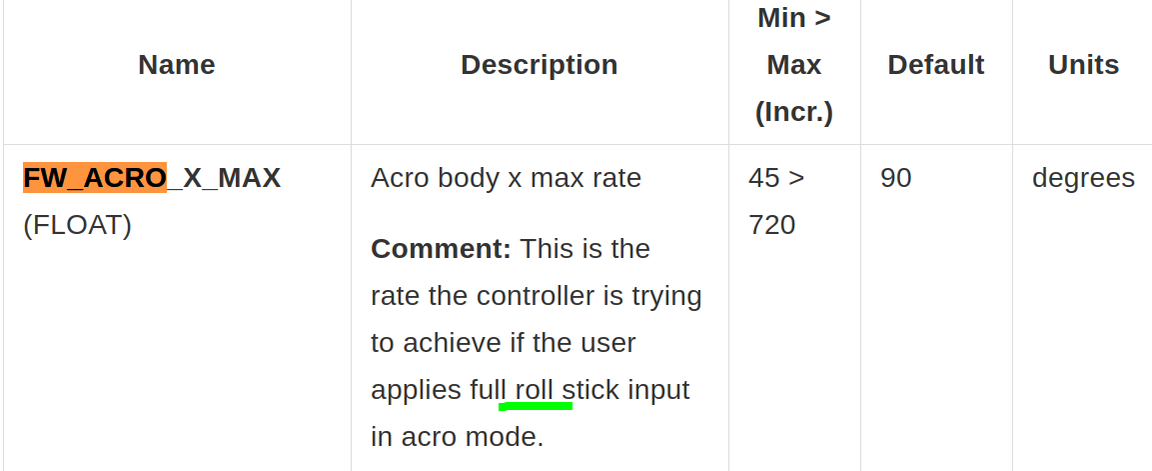
\includegraphics[width=0.48\textwidth]{pictures/parameter1.png}
  }
  \subfigure[y and z]{
      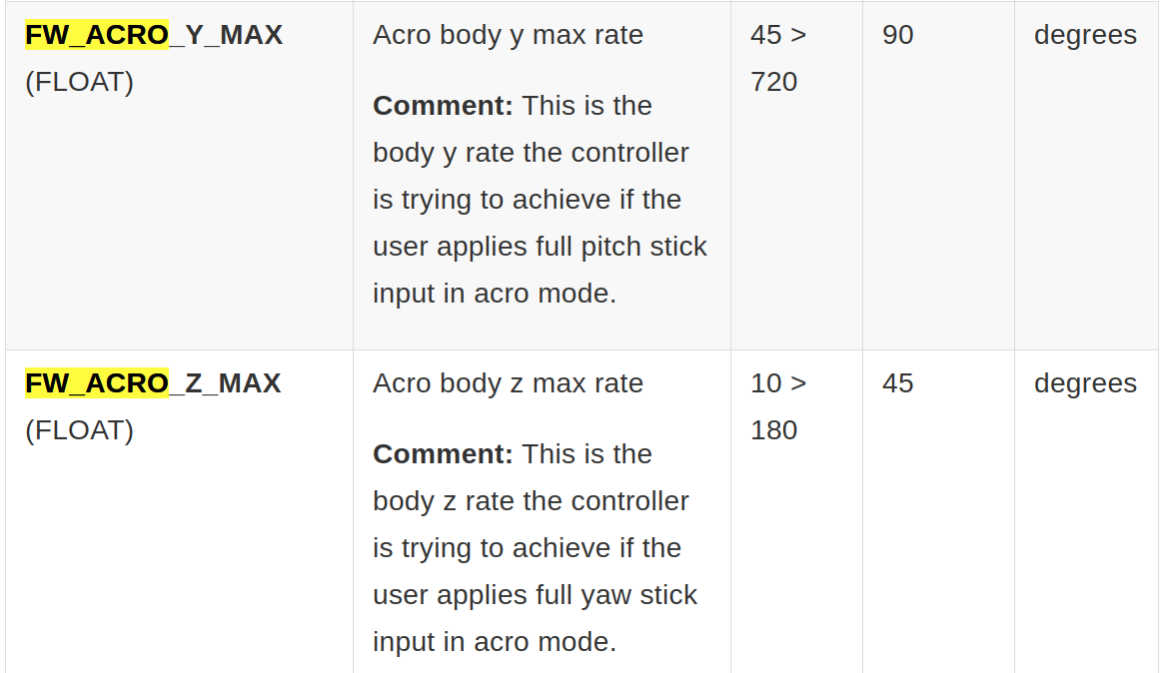
\includegraphics[width=0.48\textwidth]{pictures/att_parameter2.png}
  }
  \caption{parameters}
  \label{fig:param}
\end{figure}
其中各个参数的描述见\ref{fig:param}, 在px4中分别对应的值为\ref{equ:config}. 实现了各个参数的初始化之后, 进行下面的处理
\begin{equation}
  \begin{split}
  roll_{bodyrateSetpoint} &= [\dot{roll} - sin(pitch_{current}) * \dot{yaw}]\\
                          &.constrained[-FW\_ACRO\_X\_MAX, FW\_ACRO\_X\_MAX] \\    
  pitch_{bodyrateSetpoint} &= [cos(roll_{current})*\dot{roll} + cos(pitch_{current}) * sin(roll_{current}) * \dot{yaw}]\\
                          &.constrained[-FW\_ACRO\_Y\_MAX, FW\_ACRO\_Y\_MAX]\\
  yaw_{bodyrateSetpoint} &= [-sin(roll_{current}) * \dot{pitch} + cos(roll_{current}) * cos(pitch_{current}) * \dot{yaw}] \\
                          &.constrained[-FW\_ACRO\_Z\_MAX, FW\_ACRO\_Z\_MAX]
  \end{split}
\end{equation}
最终将上面约束过的体变化率当做姿态的设定值, 发布给下面的控制器以及执行器
\begin{equation}
  \begin{split}
    roll_{setpoint} &= roll_{bodyrateSetpoint} \\
    pitch_{setpoint} &= pitch_{bodyrateSetpoint} \\
    yaw_{setpoint} &= yaw_{bodyrateSetpoint}  
  \end{split}
\end{equation}
\subsection{欧拉角, 四元数的相互转换}
\subsubsection{欧拉角转换为四元数}

\begin{lstlisting}[title=欧拉角转换为四元数]
  void euler_2_quaternion(float angle[3], float quat[4])
  {
      // q0 q1 q2 q3
      // w x y z
      double cosPhi_2 = cos(double(angle[0]) / 2.0);
      double sinPhi_2 = sin(double(angle[0]) / 2.0);
      double cosTheta_2 = cos(double(angle[1]) / 2.0);
      double sinTheta_2 = sin(double(angle[1]) / 2.0);
      double cosPsi_2 = cos(double(angle[2]) / 2.0);
      double sinPsi_2 = sin(double(angle[2]) / 2.0);
      
      quat[0] = float(cosPhi_2 * cosTheta_2 * cosPsi_2 + sinPhi_2 * sinTheta_2 * sinPsi_2);
      quat[1] = float(sinPhi_2 * cosTheta_2 * cosPsi_2 - cosPhi_2 * sinTheta_2 * sinPsi_2);
      quat[2] = float(cosPhi_2 * sinTheta_2 * cosPsi_2 + sinPhi_2 * cosTheta_2 * sinPsi_2);
      quat[3] = float(cosPhi_2 * cosTheta_2 * sinPsi_2 - sinPhi_2 * sinTheta_2 * cosPsi_2);
  }  
\end{lstlisting}

\subsubsection{四元数转换为欧拉角}
\begin{lstlisting}[title=四元数转换为欧拉角]
  Quaternion(const Euler<Type> &euler)
    {
        Quaternion &q = *this;
    
        Type cosPhi_2 = Type(cos(euler.phi() / Type(2)));
        Type cosTheta_2 = Type(cos(euler.theta() / Type(2)));
        Type cosPsi_2 = Type(cos(euler.psi() / Type(2)));
        Type sinPhi_2 = Type(sin(euler.phi() / Type(2)));
        Type sinTheta_2 = Type(sin(euler.theta() / Type(2)));
        Type sinPsi_2 = Type(sin(euler.psi() / Type(2)));
        q(0) = cosPhi_2 * cosTheta_2 * cosPsi_2 +
               sinPhi_2 * sinTheta_2 * sinPsi_2;
        q(1) = sinPhi_2 * cosTheta_2 * cosPsi_2 -
               cosPhi_2 * sinTheta_2 * sinPsi_2;
        q(2) = cosPhi_2 * sinTheta_2 * cosPsi_2 +
               sinPhi_2 * cosTheta_2 * sinPsi_2;
        q(3) = cosPhi_2 * cosTheta_2 * sinPsi_2 -
               sinPhi_2 * sinTheta_2 * cosPsi_2;
}
\end{lstlisting}

\subsection{针对offboard对px4的更改}
在 \textcolor{red}{$fw\_att\_control.cpp$} 控制器中, 对yaw重新计算的时候, 使用的是 $roll_{setpoint}$ 而不是根据当前的roll进行两次约束之后得到的结果. 同时
也去掉$cos(pitch_{current})$这一项.

\section{RC control}
\subsection{raspberry's handled logic and px4's receiver}
树莓派的控制指令以mavlink消息$(MAVLINK_MSG_ID_RC_CHANNELS_OVERRIDE = 70)$进入到px4内部, 处理函数名字为:
\begin{lstlisting}[title=mavlink处理函数声明体]
    // Firmware/src/modules/mavlink/mavlink_receiver.cpp
    void MavlinkReceiver::handle_message(mavlink_message_t *msg);
\end{lstlisting}
\par 处理函数内部会对信息进行解码处理,得到18个通道(channels)的值,并且赋值给 $input\_rc\_s$ rc{}变量, 之后进行
有效性的处理(判断值18个通道的值是否为65535或者是0, 若是, 则该通道的值变为0; 反之, 该通道的值不变,且更新$rc.channel\_count$的值),
处理之后, 使用发布器 $\_rc\_pub$ 将该变量发布到 \\ $ORB\_ID(input\_rc)$话题上(定义发布器的时候, 会设置到PublicationMulti机制, 实例化会有一个优先级的赋值, 可以参见\textcolor{red}{需要补充} )
树莓派发送的四个值占用前四个通道,这个四个通道对应的顺序和遥控器对应指令的通道是不一样的 $(roll = 1 , pitch = 2, throttle = 3, yaw = 4)$.
\begin{lstlisting}[title=$input\_rc\_s$结构体的定义]
    struct input_rc_s {
        uint64_t timestamp;
        uint64_t timestamp_last_signal;
        uint32_t channel_count;
        int32_t rssi;
        uint16_t rc_lost_frame_count;
        uint16_t rc_total_frame_count;
        uint16_t rc_ppm_frame_length;
        uint16_t values[18];
        bool rc_failsafe;
        bool rc_lost;
        uint8_t input_source;
        uint8_t _padding0[3]; // required for logger
    }
    // publisher declaration 
    uORB::PublicationMulti<input_rc_s>			_rc_pub{ORB_ID(input_rc), ORB_PRIO_LOW};
\end{lstlisting}
\begin{lstlisting}[title=树莓派以及固件通道定义]
    // raspberry
    #define PITCH_CHANNEL 		1
    #define ROLL_CHANNEL 		2
    #define YAW_CHANNEL 		3
    #define THROTTLE_CHANNEL 	4
    
    // px4
    #define PITCH_CHANNEL 		1
    #define ROLL_CHANNEL 		2
    #define YAW_CHANNEL 		3
    #define THROTTLE_CHANNEL 	4
\end{lstlisting}

\subsection{其他部分的订阅}

mavlink接收函数拿到数据之后,进行一些处理之后, 将数据publish出去。在$rc\_update$中进行订阅
(multi publish 及其 subscribe 机制在后续文章中进行讲解),订阅器定义如下:
\begin{lstlisting}[title=订阅器的声明定义]
    // src/modules/sensors/rc_update.h
    uORB::Subscription	_rc_sub{ORB_ID(input_rc)};				/**< raw rc channels data subscription */
\end{lstlisting}

在源文件中$rc\_poll\ api$中进行更新获取该变量的值,再进行一些逻辑标志位的检索,
最后对其进行第二次的有效性检测(将每个通道的值约束到某一个固定的区间, 类似constrained()函数; trim操作, 
准备数据为manual id publish做准备), 再一次更新元素的值. 更新后的值处理.
\begin{itemize}
    \item [(1)] 发布到 ORB\_ID(rc\_channels) 话题上面.
    \item [(2)] 将 struct manual\_control\_setpoint\_s manual = {} 数据进行约束到[-1.0f, 1.0f]之间更新到该变量中,继而 发布到 ORB\_ID(manual\_control\_setpoint) 消息上.
    \item [(3)] 将第二次发布得到的 manual 变量, 赋值给 actuator\_group\_3.control 数组, 发布到\\ ORB\_ID(actuator\_controls\_3)消息上.
\end{itemize}

我们真正关心的消息topic应该是$(1\>, 2\>)$, 也就是 $ORB\_ID(rc\_channels)$ 和 $ORB\_ID(manual\_control\_setpoint)$, 
其中 $ORB\_ID(rc\_channels)$ 会被作用到PWM(遥控器和接收机的通信方式)上,所以,我们只需要关心的就是\\ $ORB\_ID(manual\_control\_setpoint)$ 消息topic即可.
\par
上述变量及其函数定义如下:
\begin{lstlisting}[title=上述变量及其函数定义]
    void RCUpdate::rc_poll(const ParameterHandles &parameter_handles);


    rc_channels_s _rc {};			/**< r/c channel data */
    orb_publish_auto(ORB_ID(rc_channels), &_rc_pub, &_rc, &instance, ORB_PRIO_DEFAULT);
    
    
    struct manual_control_setpoint_s manual = {};
    orb_publish_auto(ORB_ID(manual_control_setpoint), &_manual_control_pub, &manual, &instance,
                ORB_PRIO_HIGH);
    
    
    /* copy from mapped manual control to control group 3 */
    struct actuator_controls_s actuator_group_3 = {};
    /* publish actuator_controls_3 topic */
    orb_publish_auto(ORB_ID(actuator_controls_3), &_actuator_group_3_pub, &actuator_group_3, &instance,
                 ORB_PRIO_DEFAULT);
\end{lstlisting}

\subsection{ORB\_ID(manual\_control\_setpoint)}
这个uORB消息, 在px4内部会被 FixedWing Position Controller , FixedWing Attitude Controller 及其他原件进行订阅使用, 
这里我们需要关心的 FixedWing Position Controller , FixedWing Attitude Controller中的使用情况.
\subsubsection{FixedWing Position Controller}
在制导控制器中, px4会根据当前的throttle期望值, 调用 内部的 TECS, 进行新的姿态设定值, 计算期望空速, pitch, 以及使用其他的逻辑来进行计算 yaw, 以及roll的设定值, 赋值给变量$\_att\_sp$, 从而在最后发布给下一层的姿态控制器. 
\begin{lstlisting}[title=计算一些姿态的设定值]
_att_sp.roll_body = _manual.y * _parameters.man_roll_max_rad;
_att_sp.yaw_body = 0;

const float deadBand = 0.06f;
float factor = 1.0f - deadBand;
float pitch = -(_manual.x + deadBand) / factor;

// calculate the demanded airspeed.
float
FixedwingPositionControl::get_demanded_airspeed()
{
	float altctrl_airspeed = 0; // the demanded airspeed.

	// neutral throttle corresponds to trim airspeed
	if (_manual.z < 0.5f) {
		// lower half of throttle is min to trim airspeed
		altctrl_airspeed = _parameters.airspeed_min +
				   (_parameters.airspeed_trim - _parameters.airspeed_min) *
				   _manual.z * 2;

	} else {
		// upper half of throttle is trim to max airspeed
		altctrl_airspeed = _parameters.airspeed_trim +
				   (_parameters.airspeed_max - _parameters.airspeed_trim) *
				   (_manual.z * 2 - 1);
	}

	return altctrl_airspeed;
}
\end{lstlisting}

\textcolor{red}{上述代码公式转换如下}

\subsubsection{FixedWing Attitude Controller}
姿态控制器拿到数据且赋值给 $\_manual$ 变量.
\begin{lstlisting}[title=高度处理逻辑]
if (_vcontrol_mode.flag_control_rattitude_enabled) {
	if (fabsf(_manual.y) > _parameters.rattitude_thres || fabsf(_manual.x) > _parameters.rattitude_thres) {
		_vcontrol_mode.flag_control_attitude_enabled = false;
	}
}
\end{lstlisting}
\par
\begin{itemize}
    \item 若该变量的y和x大于 $\_parameters.rattitude\_thres$ 参数的值, 则 $flag\_control\_attitude\_enabled = false$, 若这个时候$flag\_control\_rates\_enabled$ 为真, 那么执行处理逻辑1; 再将值发布到\\$ORB\_ID(vehicle\_rates\_setpoint)$消息上, 进行下一步的处理.
    \item 若该变量的y和x小于等于 $\_parameters.rattitude\_thres$ 参数的值, 则 $flag\_control\_attitude\_enabled = true$, 执行处理逻辑2, 将值publish到 $\_attitude\_setpoint\_id$ 上面(这个topic就对应offboard从mavros发送到px4的控制逻辑层)
    \item 若不符合上面两个逻辑, 直接执行处理逻辑3, 将控制指令直接发布给执行器. 将值publish到 \\ $\_attitude\_setpoint\_id$ 上
\end{itemize}
\begin{lstlisting}[title=处理逻辑1]  
    _rates_sp.roll = _manual.y * _parameters.acro_max_x_rate_rad;
    _rates_sp.pitch = -_manual.x * _parameters.acro_max_y_rate_rad;
    _rates_sp.yaw = _manual.r * _parameters.acro_max_z_rate_rad;
    _rates_sp.thrust_body[0] = _manual.z;        
\end{lstlisting}
\begin{lstlisting}[title=处理逻辑2]  
    // STABILIZED mode generate the attitude setpoint from manual user inputs
					_att_sp.timestamp = hrt_absolute_time();

					// calculate the setpoints 
					_att_sp.roll_body = _manual.y * _parameters.man_roll_max + _parameters.rollsp_offset_rad;
					_att_sp.roll_body = math::constrain(_att_sp.roll_body, -_parameters.man_roll_max, _parameters.man_roll_max);
					_att_sp.pitch_body = -_manual.x * _parameters.man_pitch_max + _parameters.pitchsp_offset_rad;
					_att_sp.pitch_body = math::constrain(_att_sp.pitch_body, -_parameters.man_pitch_max, _parameters.man_pitch_max);
					_att_sp.yaw_body = 0.0f;
					_att_sp.thrust_body[0] = _manual.z;

					// get the Quatf
					Quatf q(Eulerf(_att_sp.roll_body, _att_sp.pitch_body, _att_sp.yaw_body));
					q.copyTo(_att_sp.q_d);
                    _att_sp.q_d_valid = true;  
                    
                    _attitude_setpoint_id = ORB_ID(vehicle_attitude_setpoint);
\end{lstlisting}
\begin{lstlisting}[title=处理逻辑3]  	
    /* manual/direct control */
    _actuators.control[actuator_controls_s::INDEX_ROLL] = _manual.y * _parameters.man_roll_scale + _parameters.trim_roll;
    _actuators.control[actuator_controls_s::INDEX_PITCH] = -_manual.x * _parameters.man_pitch_scale + _parameters.trim_pitch;
    _actuators.control[actuator_controls_s::INDEX_YAW] = _manual.r * _parameters.man_yaw_scale + _parameters.trim_yaw;
    _actuators.control[actuator_controls_s::INDEX_THROTTLE] = _manual.z;

    _actuators_id = ORB_ID(actuator_controls_0);
\end{lstlisting}

\begin{lstlisting}[title=$\_attitude\_setpoint\_id$]
_attitude_setpoint_id = ORB_ID(vehicle_attitude_setpoint);
\end{lstlisting}

\subsection{Low pass filter}
\begin{lstlisting}[title=Low pass filter from px4]
    float LowPassFilter2p::apply(float sample)
{
	// do the filtering
	float delay_element_0 = sample - _delay_element_1 * _a1 - _delay_element_2 * _a2;

	if (!PX4_ISFINITE(delay_element_0)) {
		// don't allow bad values to propagate via the filter
		delay_element_0 = sample;
	}

	const float output = delay_element_0 * _b0 + _delay_element_1 * _b1 + _delay_element_2 * _b2;

	_delay_element_2 = _delay_element_1;
	_delay_element_1 = delay_element_0;

	// return the value. Should be no need to check limits
	return output;
}
\end{lstlisting}
    
    \clearpage
    \chapter{前备知识}
\section{The centrifugal force 离心力}
    当物体在做非直线运动时(非牛顿环境,例如:圆周运动或转弯运动),
因物体一定有本身的质量存在,
质量造成的惯性会强迫物体继续朝着运动轨迹的切线方向(原来那一瞬间前进的直线方向)前进,
而非顺着接下来转弯过去的方向走。
\par 若这个在做非直线运动的物体(例如:车)上有乘客的话,乘客由于同样随着车子做转弯运动,
会受到车子向乘客提供的向心力,但是若以乘客为参照系,由于该参照系为非惯性系,
他会受到与他相对静止的车子给他的一个指向圆心的向心力作用,
但同时他也会给车子一个反向等大,由圆心指向外的力,就好像没有车子他就要被甩出去一样,这个力就是所谓的离心力。
\clearpage
 
\section{航向角和偏航角以及升力}
    \begin{itemize}
    \item[(1)] 航向角是质心沿着速度方向在水平面上的投影与预定轨迹的切线方向之间的夹角, 记为$\chi$; \\ 偏航角是质心沿着机头方向在水平面上的投影与预定轨迹的切线方向之间的夹角, 记为 $\psi$.\\
    航向角$\chi$是地速相对于$i^{i}$(正北)方向的偏移角度, 偏航角$\psi$是空速方向; \\在没有风的情况下, 偏航角和航向角是相等的
    \item[(2)] 升力是垂直副翼向上的
    \item[(3)] roll的大小和方向: 机体坐标系OZb轴与通过机体OXb轴的铅垂面间的夹角,机体向右滚为正,反之为负。
    \item[(4)] $\gamma$是 地速方向和水平方向的夹角
    \item[(5)] 圆周运动的半径, 线速度, 以及角速度三者之间的关系: $v = r \omega$
\end{itemize}
\clearpage


    \clearpage
    \section{raspberry}

\subsection{开机自启动程序sample}
在文件 $~/.config$ 文件下找到autostart文件夹, 如如果没有就新创建一个。在该文件夹下创建一个$xxx.desktop$文件,文件名自拟,后缀必须是desktop,文件内容如下:
\begin{lstlisting}[title=xxx.desktop]
    [Desktop Entry]
    Name=test
    Comment=Python Program
    Exec=python /home/pi/test.py
    Icon=/home/pi/python_games/4row_black.png
    Terminal=false
    MultipleArgs=false
    Type=Application
    Categories=Application;Development;
    StartupNotify=true
\end{lstlisting}

\begin{itemize}
    \item  Desktop Entry: 每个desktop文件都以这个标签开始,说明这是一个Desktop Entry文件
    \item  Name=python( 程序名称(必须),这里以创建一个Firefox的快捷方式为例)
    \item  Comment=Python program(程序描述 可选)
    \item  Exec=python3 wifitz.py(程序的启动命令(必选),可以带参数运行,当下面的Type为Application,此项有效. 这里是中端执行的命令,路径应该是绝对路径)
    \item  Icon=$/home/pi/python\_games/4row_arrow.png$(设置快捷方式的图标(可选),可以从系统其他地方直接法制个图标路径过来)
    \item  Terminal = false 是否在终端中运行(可选),当Type为Application,此项有效
    \item  Type = Application desktop的类型(必选),常见值有“Application”和“Link”
    \item  Categories = GNOME;Application;Network; 注明在菜单栏中显示的类别(可选)
\end{itemize}
Name、Comment、Icon可以自定,表示启动项的名称、备注和图标。
Exec表示调用的指令,和在终端输入运行脚本的指令格式一致。
如果你的树莓派没有png图标,那么就和我一样,找到 $python\_game$ 文件夹,那里有几个简单的图标可以现成拿来使用。之后再次$sudo \hspace{0.5em} reboot$

重启成功后,在linux终端使用命令\textcolor{red}{$ps \hspace{0.5em} aux$}查看当前运行的所有程序,
如果程序正常启动,可以在这里找到.

\par 如果需要启动多个程序,我试过用上述方法添加三个.desktop文件,结果失败了;
所以,如果需要启动多个程序,建议创建一个.sh脚本文件,将
多个程序的终端启动命令添加到.sh文件中,然后将上述第三步中的第4行改为Exec=./filename.sh。接下来执行第4步和第5步查看执行结果,
我这里能够成功启动三个python程序,
\textcolor{red}{本方法是利用树莓派进入桌面后再自动启动程序的方式来实现自动启动,所以需要等桌面加载完成后才启动,等待的时间相对较长一些}
这个方法测试失败!!!
\subsection{几种开机自启动的方法}
之前在树莓派上写的程序,都是通过ssh连接后在控制台上用命令行启动的,这种方式适合测试和调试,
完善好程序后,比较好的方法是把程序设置为开机自启动,
这样树莓派一上电就开始运行程序。查阅网上的资料,主要有三种方法,
% \url{https://blog.csdn.net/wangzhenyang2/article/details/80215149?utm_medium=distribute.pc_relevant.none-task-blog-BlogCommendFromMachineLearnPai2-1.nonecase&depth_1-utm_source=distribute.pc_relevant.none-task-blog-BlogCommendFromMachineLearnPai2-1.nonecase}
\par \href{https://blog.csdn.net/wangzhenyang2/article/details/80215149?utm_medium=distribute.pc_relevant.none-task-blog-BlogCommendFromMachineLearnPai2-1.nonecase&depth_1-utm_source=distribute.pc_relevant.none-task-blog-BlogCommendFromMachineLearnPai2-1.nonecase}{博客地址}
\begin{itemize}
    \item [1.] 是在$rc.local$添加启动项
    \item [2.] 是在$~/.config/autostart$中添加桌面启动应用
    \item [3.] 是在$/etc/init.d/$中添加服务项
    \item [4.] 使用systemctl设置服务
\end{itemize}
测试代码如下:
\begin{lstlisting}[title=UDP测试代码]
    #!/usr/bin/python
    import socket
    import time
    
    HOST='192.168.64.136'
    PORT=9999
    
    server=socket.socket(socket.AF_INET,socket.SOCK_DGRAM)
    server.connect((HOST,PORT))
    data='123'
    
    try:
        while True:
            server.sendall(data.encode(encoding='utf-8'))
            time.sleep(1)
    except:
        server.close()
\end{lstlisting}


\end{document}
